\documentclass{standalone}
\usepackage{graphicx}	
\usepackage{amssymb, amsmath}
\usepackage{color}

\usepackage{tikz}
\usetikzlibrary{intersections, backgrounds, math}
\usepackage{pgfmath}

\definecolor{light}{RGB}{220, 188, 188}
\definecolor{mid}{RGB}{185, 124, 124}
\definecolor{dark}{RGB}{143, 39, 39}
\definecolor{highlight}{RGB}{180, 31, 180}
\definecolor{gray10}{gray}{0.1}
\definecolor{gray20}{gray}{0.2}
\definecolor{gray30}{gray}{0.3}
\definecolor{gray40}{gray}{0.4}
\definecolor{gray60}{gray}{0.6}
\definecolor{gray70}{gray}{0.7}
\definecolor{gray80}{gray}{0.8}
\definecolor{gray90}{gray}{0.9}
\definecolor{gray95}{gray}{0.95}


\begin{document}

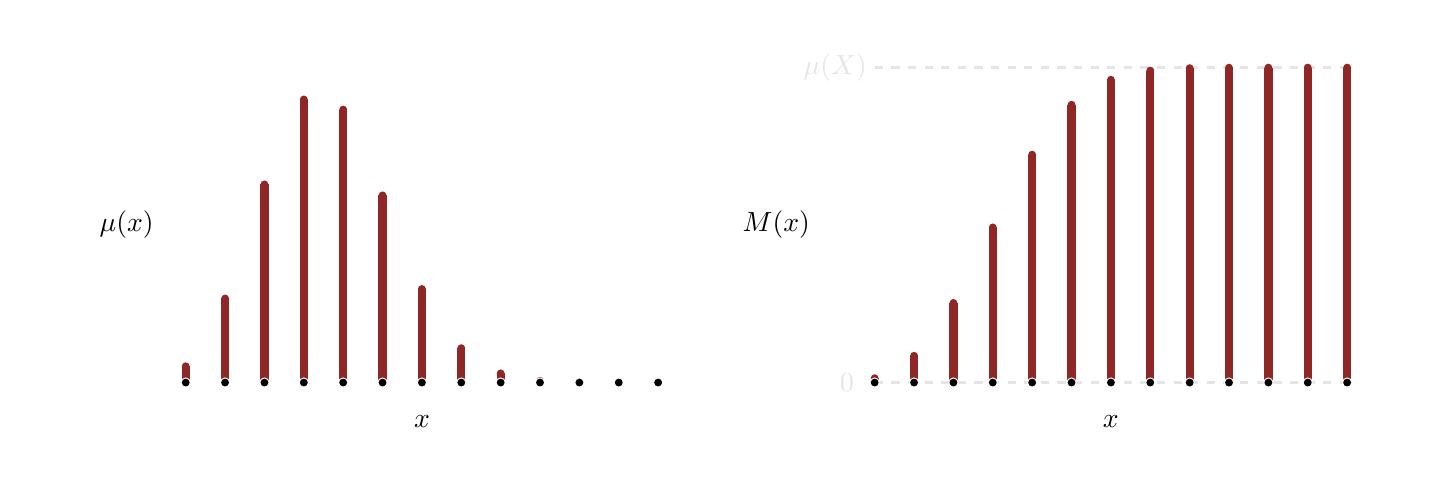
\begin{tikzpicture}[scale=1]
  \begin{scope}[shift={(0, 0)}]
    \draw[white] (-5, -3) rectangle (3.75, 2.5);
    
    \foreach [count=\n] \m in {0.013841, 0.071184, 0.167790, 0.239700, 0.231140, 0.158496, 0.079248, 0.029111, 0.007798, 0.001485, 0.000191, 0.000015, 0.000001} {
      \pgfmathsetmacro{\x}{0.5 * ( (\n - 1) - 6)};
      \draw[dark, line width=3] (\x, -2) -- (\x, {(15 * \m - 2)});
      \fill[dark] (\x, {(15 * \m - 2)}) circle (0.05);
      \fill[white] (\x, -2) circle (0.065);
      \fill[black] (\x, -2) circle (0.05);
    }
 
    \node at (0, -2.5) { $x$ };
    \node at (-3.75, 0) { $\mu(x)$ };
  \end{scope}
  
  \begin{scope}[shift={(8.75, 0)}]
    \draw[white] (-5, -3) rectangle (3.75, 2.5);
    
    \draw[gray90, dashed, line width=1] (-3, -2) -- (3, -2);
    \node[gray90] at (-3.35, -2) { $0$ };
    
    \draw[gray90, dashed, line width=1] (-3, 2) -- (3, 2);
    \node[gray90] at (-3.5, 2) { $\mu(X)$ };
    
    \foreach [count=\n] \m in {0.013841, 0.085025, 0.252815, 0.492516, 0.723655, 0.882151, 0.961399, 0.990511, 0.998308, 0.999794, 0.999985, 0.999999, 1.000000} {
      \pgfmathsetmacro{\x}{0.5 * ( (\n - 1) - 6)};
      \draw[dark, line width=3] (\x, -2) -- (\x, {(4 * \m - 2)});
      \fill[dark] (\x, {(4 * \m - 2)}) circle (0.05);
      \fill[white] (\x, -2) circle (0.065);
      \fill[black] (\x, -2) circle (0.05);
    }
      
    \node at (0, -2.5) { $x$ };
    \node at (-4.25, 0) { $M(x)$ };
  \end{scope}
  
\end{tikzpicture}

\end{document}  